\documentclass[12pt,letterpaper]{article}
\usepackage[utf8]{inputenc}
\usepackage{natbib}
\usepackage{graphicx}
\usepackage{indentfirst}
\usepackage{indentfirst}
\usepackage[left=3cm,right=2cm,top=2cm,bottom=3cm]{geometry}

\usepackage{lipsum}

\setlength{\parindent}{2cm}
\setlength{\parskip}{\baselineskip}
\renewcommand{\baselinestretch}{1.5}

\renewcommand\contentsname{Índice de contenidos}
\renewcommand\refname{Referencias}

\begin{document}

\newpage
\vspace*{-.5cm}
\begin{picture}(18,4)(0,40)
	\put(350,-20){
\includegraphics[scale=.25]{images/LogoUsach.pdf}}
\end{picture}

\sloppy
\thispagestyle{empty}
\vspace*{-1.6cm}

\begin{center}
	{\bf \mbox{\large UNIVERSIDAD DE SANTIAGO DE CHILE}}\\
	{\bf \mbox{FACULTAD DE INGENIER\'IA}}\\
	{\bf \mbox{DEPARTAMENTO DE INGENIER\'IA INFORM\'ATICA}}\\
\end{center}

	\vspace*{3cm}
	\par
	\vspace{1cm}
	\begin{center}
	\large
		Organización de Computadores\\Laboratorio \#1
	\end{center}
	\vspace{3cm}
	\begin{flushright}
		\begin{tabular}[t]{l l}
			Integrantes: & Nestor Mora \\
			             & Cristian Espinoza \\
			Profesor(a): & Nicolas Hidalgo \\
						 & Erika Rosas \\
			Ayudante: & Felipe Fuentes\\

		\end{tabular}
	\end{flushright}
	\begin{center}
		\vspace{3cm}
		Lunes, 6 de Octubre de 2014
	\end{center}



\newpage
\tableofcontents
\thispagestyle{empty}

\newpage
\renewcommand{\thepage}{\arabic{page}}
\setcounter{page}{1}
\section{Introducción}
El presente informe, detalla elaboración del Laboratorio 1 del ramo Organización de Computadores, el cual consiste en la producción de una aplicación que desarrolle el logaritmo natural de un número, pero resuelto a través del uso de la Serie de Taylor.

El objetivo principal es disminuir el tiempo de ejecución de la aplicación.

Los objetivos específicos son la elaboración de la aplicación que desarrolle la serie de Taylor para resolver el logaritmo natural de un número, detectar los hazards y la disminución en la cantidad de tareas realizadas en el proceso de calcular la serie.

Para disminuir el tiempo de ejecución de la aplicación, se ha procedido a considerar los hazards y a través del uso de pipeline, reordenar algunas instrucciones para que no exista la necesidad de esperar los resultados.
\newpage
\section{Marco Teórico}
\subsection{Serie de Taylor}
La Serie de Taylor es una serie funcional y surge de una ecuación en la cual se puede encontrar una solución aproximada a una función.

Ésta sirve para conseguir una aproximación del valor de una función en un punto.

\subsection{Pipeline}
Es una técnica de implementación en la cual múltiples instrucciones están traslapadas en la ejecución. Esto sirve para disminuir el tiempo de ejecución de un programa.

\subsection{Getopt}
Es una biblioteca de funciónes C, utilizado para analizar las opciones de línea de comandos .
También es el nombre de un programa de Unix para analizar los argumentos de línea de comandos en shell scripts.%agregar referencia http://en.wikipedia.org/wiki/Getopt
\newpage
\section{Desarrollo}
\subsection{Gráfico de iteraciones}
\begin{picture}(100,175)(0,40)
	\put(-50,5){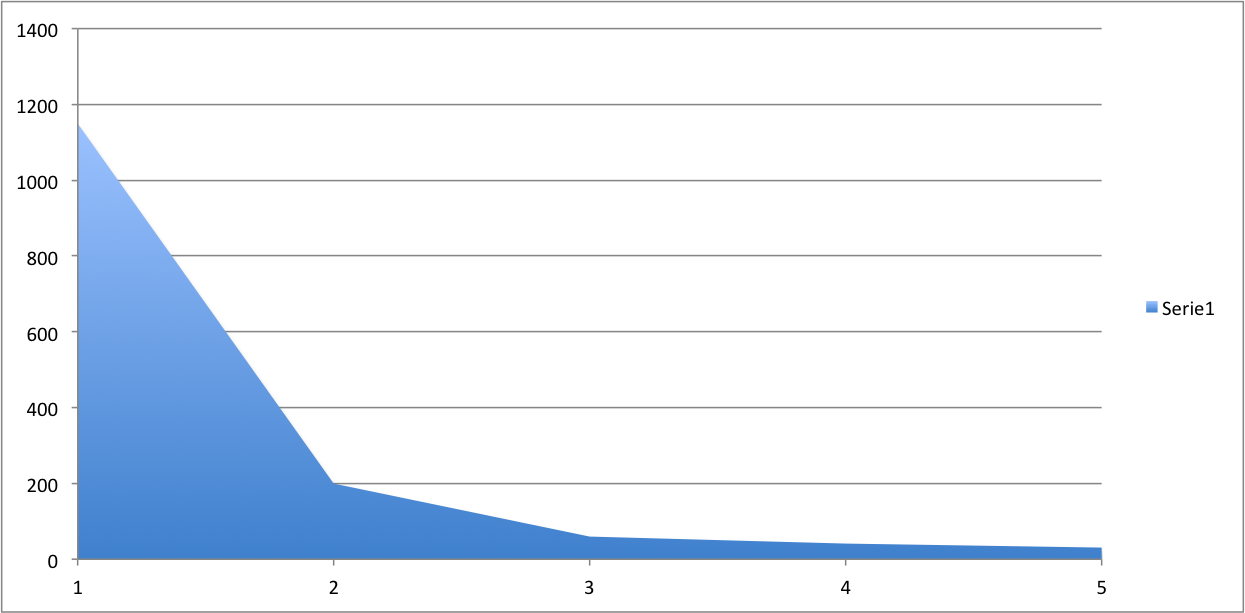
\includegraphics[scale=.75]{images/graf1.png}}
\end{picture}
\subsection{Descripción del problema}
Se pide realizar la Serie de Taylor para resolver el logaritmo natural de un número, para luego ir mejorando el código, y después de eso, a través del uso de pipeline ir disminuyendo el tiempo de ejecución de este.

\subsection{Primer Paso - main0.c}
Lo primero que se realizó, fue escribir el programa tal cual se presentó en el ejemplo, ésto es definiendo el valor de las constantes que se encuentran en el desarrollo de la serie de taylor, realizando la fracción en la función de logaritmo natural, para luego realizar las multiplicaciones de estas fracciones con las constantes.

\subsection{Segundo Paso - main1.c}
Lo segundo en hacer fue colocar el desarrollo de la fracción en la parte principal del programa, para así no calcularlo en cada multiplicación de la función logaritmo, sino que solo multiplicar el resultado ya obtenido para así calcular la serie de taylor, dentro de este mismo paso, se decidió aumentar la cantidad de constantes y por lo tanto la cantidad de multiplicaciones realizadas al calcular la serie de taylor, ésto para que el valor obtenido sea más cercano al valor real del logaritmo natural, aquí se presenta la primera gran problemática, ya que al aumentar demasiado la cantidad de constantes, el programa demora más tiempo al calcular el valor, así que se decide trabajar solo con 20 constantes.

\subsection{Tercer Paso - main2.c}
Se decide trabajar con los valores ya calculados, es decir, ir agregando a la multiplicación ya realizada, el valor que debe ser multiplicado después, disminuyendo así la cantidad de multiplicaciones que deben realizarse.

\subsection{Cuarto Paso - main3.c}
Del programa anterior, se decidió que en la linea "retorno += c2 * x_2nplus1;" se están realizando 2 operaciones, una multiplicación y una suma, ademas de tener dependencia de la linea anterior "x_2nplus1 *= x_cuad;", considerando esto se decidió aumentar en una linea, y en ella depositar en una variable temporal   "temp=c2 * x_2nplus1;" con ello se manejan las dependencias, reduciendo el tiempo de ejecución.


\subsection{Quinto Paso - main4.c}
En el quinto paso se decidió cambiar la función que va ocupando los valores ya calculados, por una función que es netamente la factorización de lo que realiza la multiplicación en la serie de taylor, ya teniendo calculados dos valores que se repetirán a lo largo de la función que son x al cuadrado y x a la cuarta.
\newpage
\section{Discusiones}
\subsection{MER: Modelo Entidad Relación}

\subsection{MR: Modelo Relacional}
\textbf{Entidades}

\begin{itemize}
\item Institución (Codigo\_institución, Nombre\_institución)
\item Carrera (Cod\_Carrera, Nombre\_Carrera)
\item Ramo (Cod\_Asig, Nombre\_Ramo, Semestre, Año)
\item Material (Cod\_Material, Visibilidad, Versión, Autor)
\end{itemize}

\textbf{Relaciones}
\begin{itemize}
\item Imparte (Codigo\_institución, Cod\_Carrera)
\item Contiene (Cod\_Carrera, Cod\_Asig)
\end{itemize}

\newpage
\section{Conclusión}
\lipsum[1-3]

\newpage
\addcontentsline{toc}{section}{Referencias}
\bibliographystyle{plain}
\bibliography{references}

\end{document}
